		\subsection{Naïves Bayes}
			Ce type de modèle est utilisé par le module \emph{langdetect} qui me sert pour la détection des langues.

			\paragraph{Introduction}
				Les modèles Naïves Bayes se basent sur le théorème de probabilité de Bayes. Il permet de déterminer la probabilité conditionnelle d'apparition d'un évènement A sachant qu'un évènement B s'est produit. Le terme naïf fait référence au fait que l'on présuppose que les évènements A et B ne sont pas corrélés.\\
				Ces techniques sont utilisées pour des modèles de classification en apprentissage supervisé.\\

				La formule mathématique de ce théorème est la suivante :
				\begin{eqnarray}\label{NBeq}
					P(A|B) &=& \frac{P(B|A)P(A)}{P(B)}
				\end{eqnarray}

			On recherche ici $P(A|B)$, c'est a dire la probabilité d'apparition d'un évènement A sachant que l'évènement B s'est produit. \\ 

			Pour ce faire nous avons besoin des données suivantes :
			\begin{itemize}
				\item $P(B|A)$ est la probabilité que l'évènement B s'est produit sachant que l'évènement A s'est produit
				\item $P(A)$ est la probabilité d'apparition de l'évènement A
				\item $P(B)$ est la probabilité d'apparition de l'évènement B
			\end{itemize}

			\paragraph{Exemples d'utilisation}
				Les exemples ci dessous vont permettre d'illustrer l'utilisation de cette technique. D'abord manuellement sur un petit jeu de données puis à l'aide d'un code pré-existant sur un autre jeu de données plus important.

				\subparagraph{Manuel}
					Dans cet exemple nous allons déterminer la probabilité qu'a un joueur d'aller sur le terrain selon les conditions météorologiques. Cette probabilité sera calculée en fonction des données récupérées lors des matchs précédents.\footnote{Les données présentées sont inventées} \\

					On recherchera ainsi la probabilité de présence sur le terrain d'un joueur selon la météo $P(A|B)$. Pour ce faire nous auront besoin de: 
					\begin{itemize}
						\item $P(A)$ Probabilité de jouer quelque soit le temps
						\item $P(B)$ Probabilité de l'évènement météorologique
						\item $P(B|A)$ Probabilité de l'évènement sachant que le joueur a été sur le terrain					
					\end{itemize}

				\begin{table}[H]
					\centering
					\captionof{table}{Données de présence sur le terrain} \label{tab:data}
					\begin{tabular}{|l|c|c|c|c|c|c|c|}
						\hline
						météo & soleil & soleil & couvert & pluie & pluie & pluie & couvert \\
						\hline
						présent & non & non & oui & oui & oui & non & oui \\
						\hline
						\hline
						météo & soleil & soleil & pluie & soleil & couvert & couvert & pluie \\
						\hline
						présent & non & oui & oui & oui & oui & oui & non \\
						\hline
					\end{tabular}
				\end{table}

				\begin{table}[H]
					\centering
					\captionof{table}{Synthèse et probabilité simple P(A) et P(B)} \label{tab:pab}
					\begin{tabular}{|l|c|c|r|}
						\hline
						météo & oui & non & $P(B)$\\
						\hline
						couvert & 4 & 0 & $4/14$\\
						\hline
						soleil & 2 & 3 & $5/14$\\
						\hline
						pluie & 3 & 2 & $5/14$\\
						\hline
						$P(A)$ & $9/14$ & $5/14$ & \\
						\hline
					\end{tabular}
				\end{table}

				On peut déterminer les probabilités de chaque météo en fonction de la présence du joueur sur le terrain P(B|A). Pour ce faire on divise le nombre d'évènements de présence du joueur lors d'un évènement météo par le nombre total d'évènements de présence du joueur

				\begin{table}[H]
					\centering
					\captionof{table}{Probabilité météo selon présence du joueur} \label{tab:pba}
					\begin{tabular}{|l|c|c|}
						\hline
						météo & P(B|oui) & P(B|non) \\
						\hline
						couvert & $4/9$ & $0/5$ \\
						\hline
						soleil & $2/9$ & $3/5$ \\
						\hline
						pluie & $3/9$ & $2/5$ \\
						\hline	
					\end{tabular}
				\end{table}

				On va maintenant calculer la probabilité qu'à un joueur d'être sur le terrain si le temps est couvert.\\
				On commence par la probabilité du oui:
				\begin{eqnarray*}
					P(A|B) &=& \frac{P(B|A)P(A)}{P(B)}\\
					P(A|B) &=& \frac{\frac{4}{9}\cdot\frac{9}{14}}{\frac{4}{14}}\\
					P(A|B) &=& \frac{\frac{4}{14}}{\frac{4}{14}}\\
					P(A|B) &=& \frac{4}{14}\cdot\frac{14}{4}\\
					P(A|B) &=& 1
				\end{eqnarray*}

				On enchaîne sur la probabilité de ne pas jouer si le temps est couvert
				\begin{eqnarray*}
					P(A|B) &=& \frac{P(B|A)P(A)}{P(B)}\\
					P(A|B) &=& \frac{\frac{0}{5}\cdot\frac{5}{14}}{\frac{4}{14}}\\
					P(A|B) &=& 0\cdot\frac{14}{4}\\
					P(A|B) &=& 0
				\end{eqnarray*}	

				On peut dire que si le temps est couvert le joueur très probablement sur le terrain			 
				On peut également déterminer la probabilité de jouer pour chaque évènement météo
				\begin{table}[H]
					\centering
					\captionof{table}{Probabilité présence du joueur selon la météo} \label{tab:pab2}
					\begin{tabular}{|l|c|c|c|}
						\hline
						météo & oui & non & plus probable\\
						\hline
						couvert & 1 & 0 & oui\\
						\hline
						soleil & 2/5 & 3/5 & non \\
						\hline
						pluie & 3/5 & 2/5 & oui \\
						\hline
					\end{tabular}
				\end{table}

				\emph{Cas polynomial}: Il est possible de déterminer la probabilité d'un évènement par rapport à plus autres. Dans ce cas, il faudra multiplier entre elles les probabilités de ces évènements selon l'apparition de l'évènement voulu.\\

				 Calcul pour un évènement (A) selon 2 autres évènements (B et C)
				 \begin{eqnarray*}
				 	P(A|BC) &=& \frac{P(B|A)P(C|A)P(A)}{P(B)P(C)}
				 \end{eqnarray*}

				\subparagraph{En code} Dans cet exemple nous allons utiliser un code existant dans la librairie python scikit-learn\cite{scikit-learn}. Ce moteur Naïves Bayes va nous permettre cette fois-ci de catégoriser des variétés d'iris selon la longueur et la largeur des pétales et des sépales. Les données proviennent cette fois-ci d'un dataset également disponible dans scikit-learn.

				Nous allons utilisé le modèle \emph{GaussianNB} de scikit-learn qui est adapté lorsque les données utilisées suivent une distribution normale. Ce qui semble être le cas pour les longueurs et largeur des sépale. 
				\begin{figure}[H]
					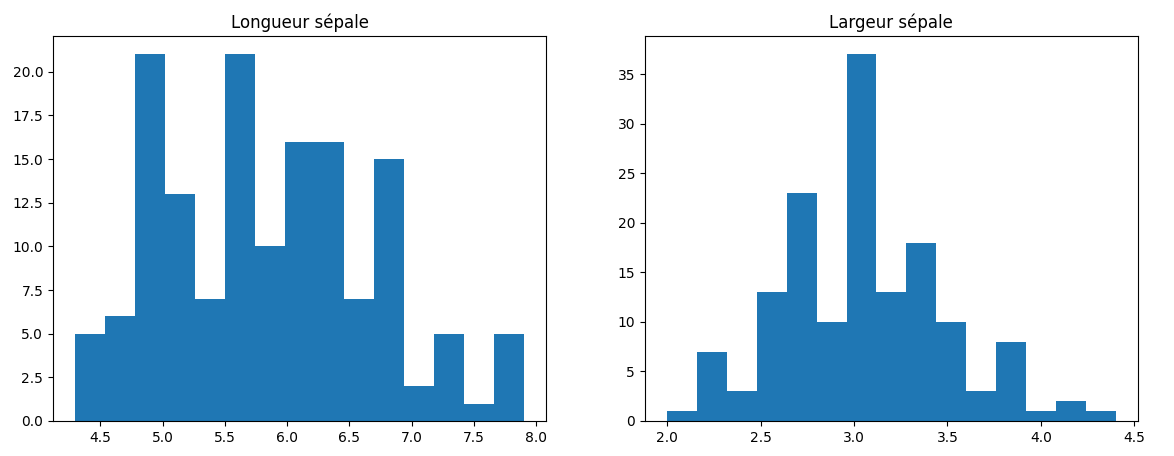
\includegraphics[width=\linewidth]{img/NBdistrib.png}
					\caption{Distribution des longueurs et largeurs des sépales}
				\end{figure}

\begin{lstlisting}[title=Progamme complet]
from sklearn.datasets import load_iris
from sklearn.model_selection import train_test_split
from sklearn.naive_bayes import GaussianNB
from sklearn.metrics import accuracy_score, confusion_matrix, ConfusionMatrixDisplay, f1_score, \
    recall_score

import matplotlib.pyplot as plt

X, y = load_iris(return_X_y=True)

X_train, X_test, y_train, y_test = train_test_split(X, y, test_size=0.33, random_state=0)
model = GaussianNB()
model.fit(X_train, y_train)

y_pred = model.predict(X_test)
precision = accuracy_score(y_pred, y_test)
recall = recall_score(y_test, y_pred, average="weighted")
f1 = f1_score(y_pred, y_test, average="weighted")

print("Precision:", precision)
print("Rappel:", recall)
print("Score F1:", f1)

plt.figure('Donnees du modele', figsize=(14, 5))
plt.subplot(1, 3, 1, title='Donnees du train set')
plt.scatter(X_train[:, 0], X_train[:, 1], c=y_train)
plt.xlabel('Sepale long.')
plt.ylabel('Sepale larg.')
plt.subplot(1, 3, 2, title='Donnees du test set')
plt.scatter(X_test[:, 0], X_test[:, 1], c=y_test)
plt.xlabel('Sepale long.')
plt.subplot(1, 3, 3, title='Donnees test apres evaluation')
plt.scatter(X_test[:, 0], X_test[:, 1], c=y_pred)
plt.xlabel('Sepale long.')
plt.show()

cm = confusion_matrix(y_test, y_pred, labels=[0, 1, 2])
disp = ConfusionMatrixDisplay(confusion_matrix=cm, display_labels=[0, 1, 2])
disp.ax_.set_title('Matrice de confusion')
disp.plot()
plt.show()

plt.figure('Distribution des donnees Iris', figsize=(14, 5))
plt.subplot(1, 2, 1, title='Longueur sepale')
plt.hist(X[:, 0], bins=15)
plt.subplot(1, 2, 2, title='Largeur sepale')
plt.hist(X[:, 1], bins=15)
plt.show()\end{lstlisting}

				Les données du dataset ont été séparés en 2 jeux, un pour l’entraînement du modèle et un pour le test. On obtient alors la représentation suivantes après entrainement et test du modèle
				\begin{figure}[H]
					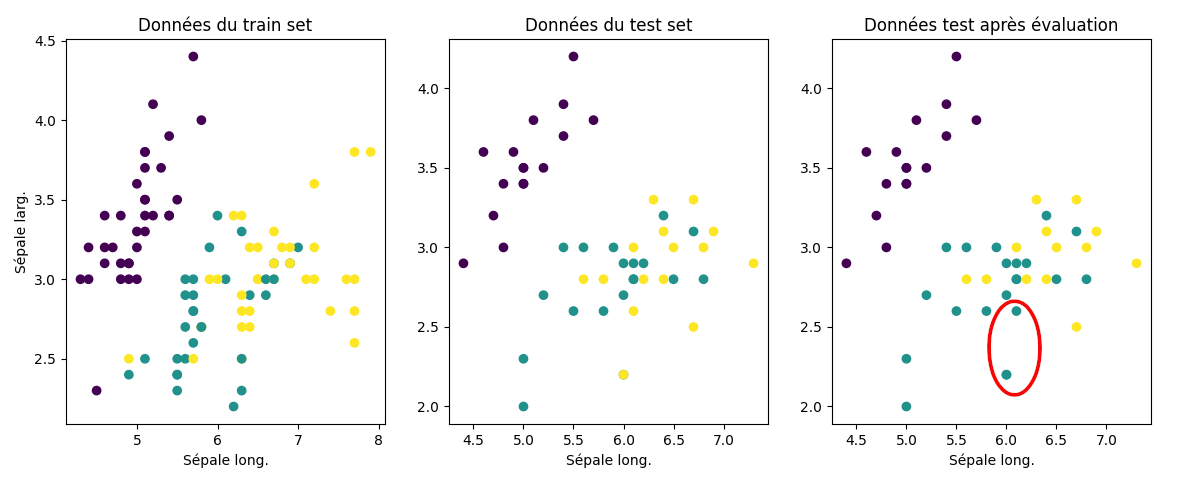
\includegraphics[width=\linewidth]{img/NBdata.png}
					\caption{Représentation des données }
				\end{figure}

				Dans les données de test nous avons 2 catégorisations qui n'ont pas été réalisées correctement. On obtient les scores suivants :
				\begin{itemize}
					\item Précision: 0.96                    \footnote{La précision est la proportion des éléments correctement identifiés sur l'ensemble des éléments prédit}
					\item Rappel: 0.96						\footnote{Le rappel est la proportion des éléments correctement identifiés sur l'ensemble des éléments de la catégorie}
					\item Score F1: 0.9604285714285714		\footnote{Le Score F1 est la moyenne harmonique calculée de la manière suivante $2*(precision*rappel)/(precision+rappel)$}
				\end{itemize}				

				\begin{figure}[H]
					\centering
					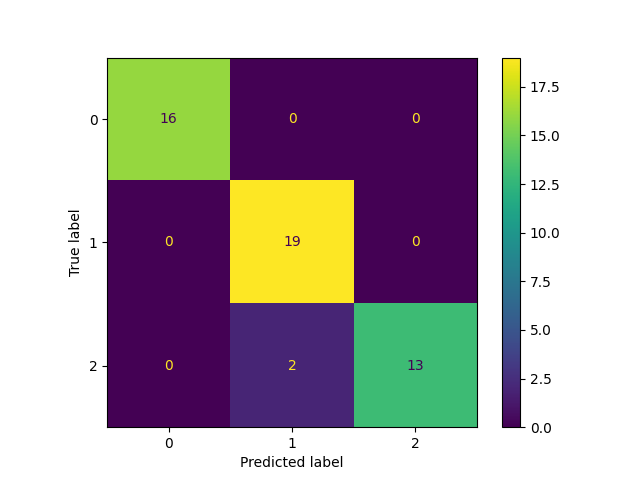
\includegraphics[scale=0.7]{img/NBmatrix.png}
					\caption{Matrice de confusion}
				\end{figure}

				A l'aide de ce modèle nous devrions avoir une 96\% de chance de déterminer la bonne variété d'iris en se basant sur la longueur et la largeur des sépales.  

			\paragraph{Avantages et inconvénients} 
				Le modèle Naïve Bayes est un modèle simple et rapide qui ne nécessite pas de grande capacités de calcul. De ce fait il permet de traiter une grande quantité de données.\\

				Cependant, les données qui lui sont fournies ne doivent pas être corrélées ce qui est rarement le cas dans les problèmes du monde réel. Ce type de modèle est limité à des problèmes de classification supervisée. Si on se fie à l'équation (\ref{NBeq}) la probabilité d'apparition de l’évènement B : P(B) ne peut pas être nulle.